\chapter{Future Improvements and Conclusions}
\label{conclusion}

\section{Future Improvements}
\label{sec:Future}

There are a number of improvements that could be made for this analysis. First and foremost, more data will mean stronger limits. The data used in this analysis represents less than $20\%$ of the total planned exposure, so the measurements will naturally become stronger with time. Figure \ref{fig:Fit3yr} shows how the $\theta_{34}$ limit will improve with \pot{18}, using the same rate only fit and assuming a modest $50\%$ reduction in the cosmic background. Even under these assumptions, \nova~will match the current best measurement from Super-K \cite{ref:SuperKSterile} of $\theta_{34} < 25^\circ (90\% \mbox{C.L.})$.
\begin{figure}[htb]
  \centering
  \begin{tabular}{c c}
    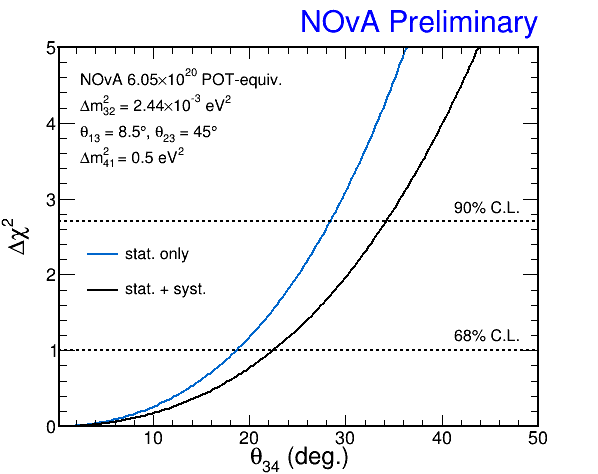
\includegraphics[width=.47\textwidth]{figures/Fits/1DTh34.png} &
    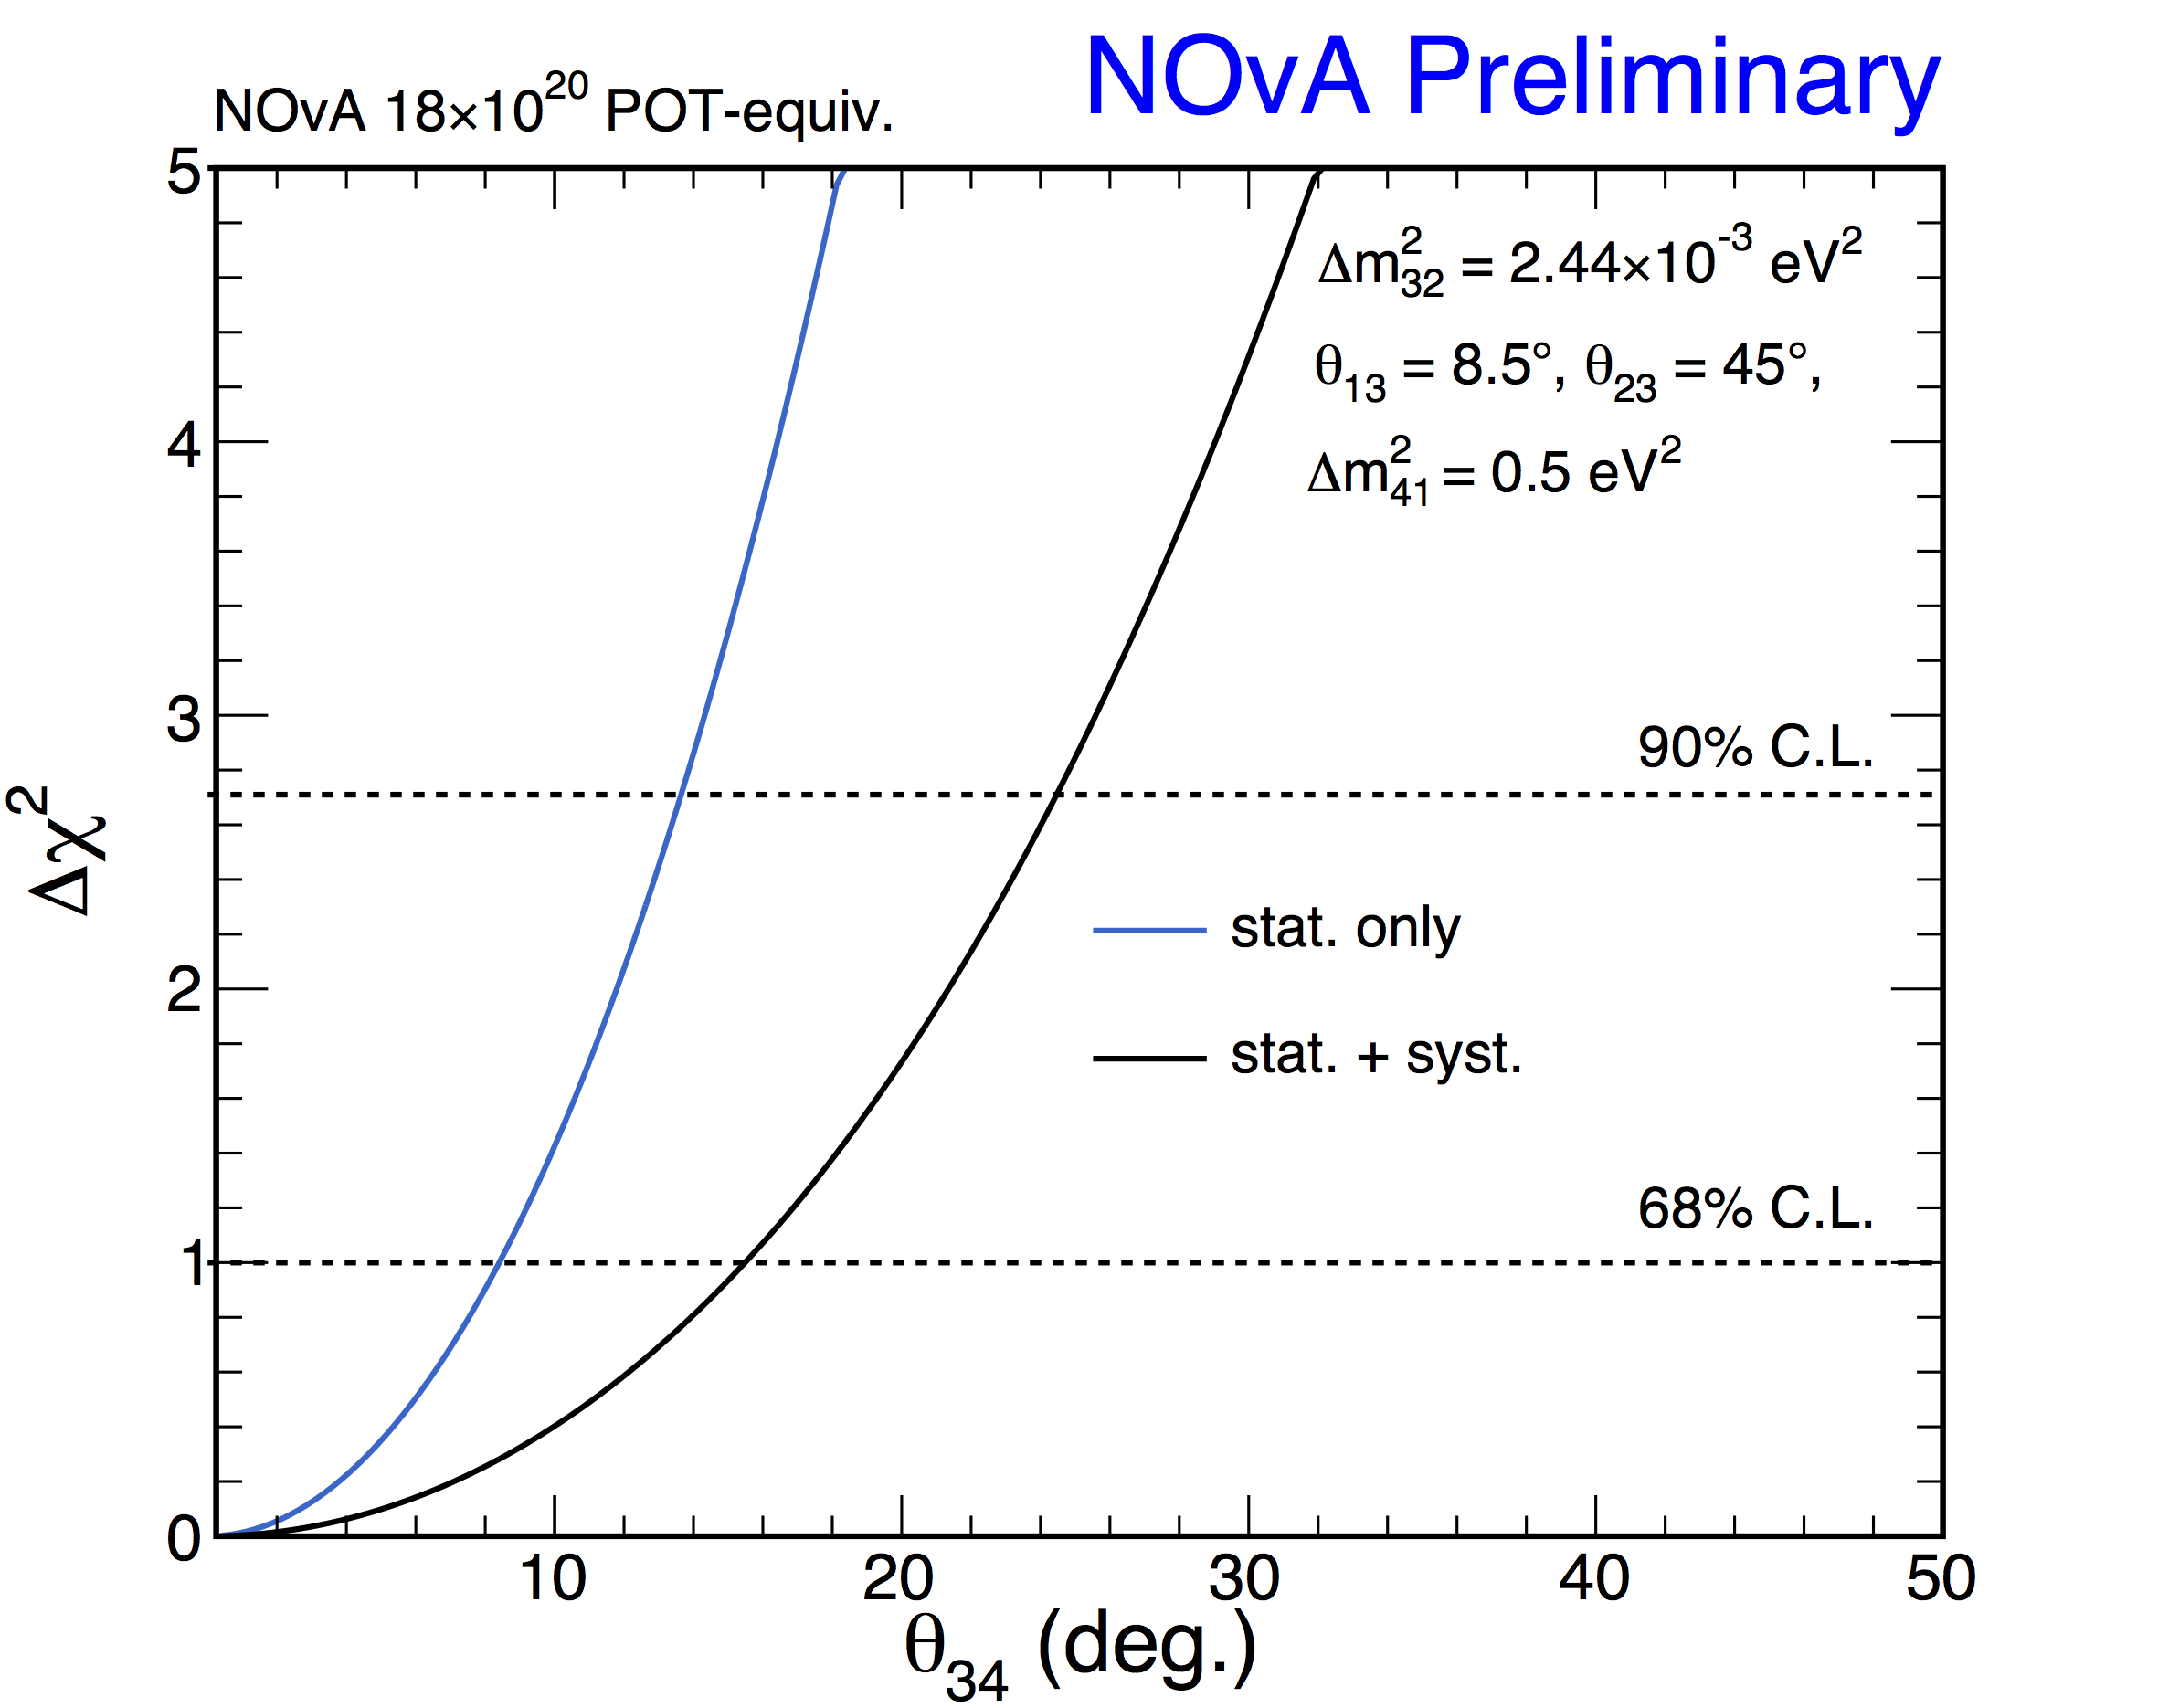
\includegraphics[width=.47\textwidth]{figures/Fits/1DTh34_3yr.png} \\
  \end{tabular}
  \caption[Projected Sensitivity for $\theta_{34}$ After \pot{18}.]{The projected sensitivity for $\theta_{34}$. The left figure shows the measurement from this analysis. The right figure shows the projected measurement after \pot{18}, and assuming a $50\%$ reduction in the cosmic background. The projected $90\%$ confidence measurement is an upper limit slightly below $25^\circ$, the current best measurement on $\theta_{34}$ from Super-K \cite{ref:SuperKSterile}.}
  \label{fig:Fit3yr}
\end{figure}

Probably the most important advance for the analysis itself would be the improvement of the cross section information, including the use of data to tune existing models and to include NC MEC events. In fact, the ND data/MC shape discrepancy was the driving force behind using the more robust rate only analysis, as opposed to a rate and shape analysis. The cross section model work, which is already underway, should improve this data/MC disagreement, at which point it will be natural to move to the shape and rate analysis. In fact, the functionality to perform a shape and rate analysis already exists and has been demonstrated, so this is the lowest hanging fruit for analysis improvements.

The neutral current selection has a number of places it could be improved. As mentioned in several sections of chapter \ref{ch:Selection}, it was discovered after selection cuts were frozen that many of the reconstructed objects used for selection had hidden preselections applied. The prongs and tracks used for containment are prime examples of this, so there are plans to move to a more reconstruction free containment. The cosmic rejection BDT also requires a reconstructed track, so there are ongoing efforts to perform the cosmic rejection in a way that relaxes this constraint, even if this means handling $0$ track events differently. Any overall improvements to the cosmic rejection could also translate into signal gains. The very harsh fiducial volume and containment cut at the top of the FD was made to remove cosmic events, so overall cosmic rejection improvements could relax these cuts and allow more signal events into the selected sample. 

The largest systematic error came from the ND data/MC discrepancy. Future analyses should improve this in two ways. First, the inclusion of NC MEC events and improvement of the cross section models should naturally improve the ND data/MC shape agreement. Even a modest $50\%$ improvement on this systematic would translate into an overall systematic error reductions of $13\%$ for the NC signal and $19\%$ for the CC background. The other improvement would come from choosing a data driven decomposition method. This would require that the systematic be evaluated in a different way as well.

One other major analysis improvement would be to increase the range of $\dmxy{1}{4}$ to higher values. It can be seen from figure \ref{fig:LOverEDm41} that this could affect the ND event rate. Consequently, this would require performing a joint oscillation parameter fit to the ND and FD data.

\section{Conclusion}
\label{sec:Conclusion}

The NC disappearance analysis presented in this dissertation searched for mixing between active and sterile neutrinos in a $3 + 1$ model. \pot{6.69} were collected at the FD, or $6.05 \times 10^{20}$ full detector equivalent POT. The results of this analysis were consistent with the no sterile neutrino mixing hypothesis and placed upper limits on the allowed values of the mixing angles and matrix elements. There are many known avenues for future improvements to the analysis, including model improvements, moving to a shape and rate analysis, gaining signal efficiency from different reconstructed objects, and performing a joint ND and FD fit. With only modest improvements, \nova~will set competitive limits on the best fit value of $\theta_{34}$ and $\Usqxy{\tau}{4}$ in a few years time. This is only the beginning of an exciting \nova~analysis!